\titlepageframe % Specific command 
%%%%%%%%%%%%%%%%%%%%%%%%%%%%%%%%%%%%%%%%%%%%%%%%%%%%%%%%%%%%%
\begin{tframe}{Introduzione}
\begin{itemize}
\item Dalla crisi del 2007 e la conseguente esplosione delle basi tra tassi di tenore differente il mercato dei derivati su tasso si è dovuto adattare a quello che è stato definito: Mondo Multi-Curva
    \begin{itemize}
    \item Esigenza di calibrare una curva di forwarding per ogni tenore
    \item Esigenza di calibrare una curva di discounting esogeno da applicare ad ogni tenore
    \end{itemize}
\item In questo contesto, poichè i collateral scambiati vengono depositati su conti che maturano interessi al tasso EONIA, la curva overnight ha assunto:
   \begin{itemize}
    \item Il compito di curva di discounting esogeno applicabile ad ogni tenore
    \item Il compito di curva di forwarding per il proprio tenore
    \end{itemize}
\item Introdurre distorsioni nella calibrazione conduce a prezzi non ragionevoli specialmente per scopi di trading, dove $1/4$ di Basis Point può fare la differenza    
\end{itemize}
\end{tframe}
%%%%%%%%%%%%%%%%%%%%%%%%%%%%%%%%%%%%%%%%%%%%%%%%%%%%%%%%%%%%%
\begin{tframe}
\begin{figure}[!h]
\centering
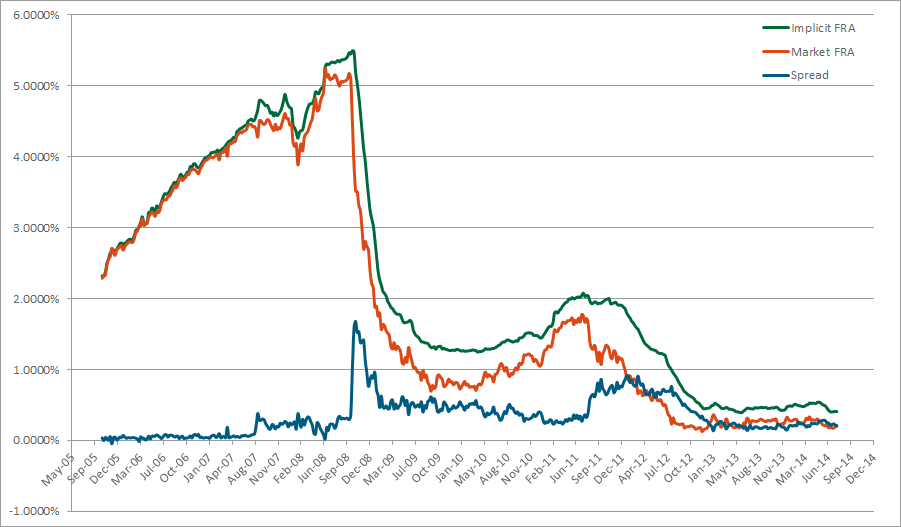
\includegraphics[width=0.8\textwidth]{basisafter.png}
\caption{Dopo l'estate del 2007 il  $3X6$ FRA implicito nei fixings di Euribor6M e Euribor3M non era più in linea con il $3X6$ FRA quotato sul mercato.}
\label{fig:basisafter}
\end{figure}
\end{tframe}
%%%%%%%%%%%%%%%%%%%%%%%%%%%%%%%%%%%%%%%%%%%%%%%%%%%%%%%%%%%%%
\begin{tframe}{Composizione curva Overnight}
\begin{itemize}
\item Il principio di coerenza di tenore e liquidità impone che la best practice per il bootstrap della curva overnight preveda l'inclusione di:
    \begin{itemize}
    \item Tutti forward ECB OIS disponibili sul mercato
    \item OIS con partenza spot fino a 60Y
    \end{itemize}
\item Tuttavia gli ECB OIS sono più liquidi degli OIS con partenza spot e, per questo motivo, gli algoritmi di calibrazione gli danno precedenza andando ad escludere i rispettivi spot OIS che coprono la stessa frazione di anno    
\end{itemize}
\end{tframe}
%%%%%%%%%%%%%%%%%%%%%%%%%%%%%%%%%%%%%%%%%%%%%%%%%%%%%%%%%%%%%
\begin{tframe}{Strumenti sovrapposti}
\begin{itemize}
\item Il principio di coerenza di tenore e liquidità impone che la best practice per il bootstrap della curva overnight preveda l'inclusione di:
    \begin{itemize}
    \item Tutti forward ECB OIS disponibili sul mercato
    \item OIS con partenza spot fino a 60Y
    \end{itemize}
\item Tuttavia gli ECB OIS sono più liquidi degli OIS con partenza spot e, per questo motivo, gli algoritmi di calibrazione gli danno precedenza andando ad escludere i rispettivi spot OIS che coprono la stessa frazione di anno 
\item In questo modo si crea una sezione di curva con strumenti sovrapposti che introduce distorsioni nella calibrazione
\end{itemize}
\end{tframe}
%%%%%%%%%%%%%%%%%%%%%%%%%%%%%%%%%%%%%%%%%%%%%%%%%%%%%%%%%%%%%
\begin{tframe}
\begin{figure}[!h]
\centering
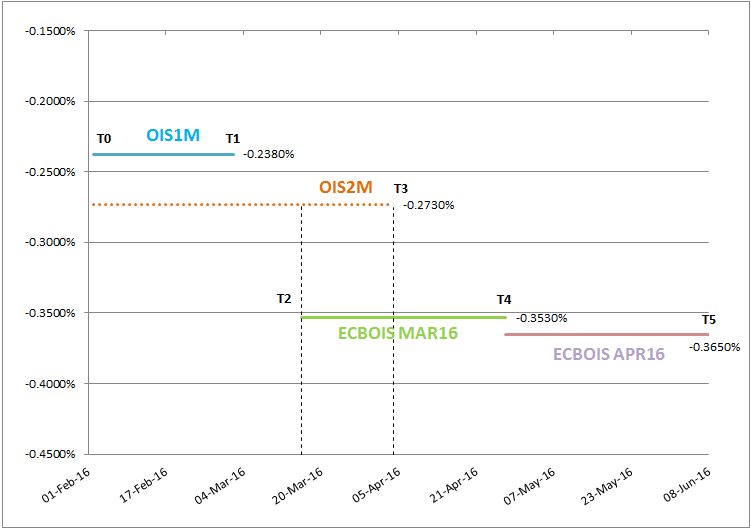
\includegraphics[width=0.75\textwidth]{overlappingsol.png}
\caption{Evidenza di strumenti sovrapposti nella curva overnight; dataset del {\it 29 Gennaio 2016}.}
\label{fig:overlappingsol}
\end{figure}
\end{tframe}
%%%%%%%%%%%%%%%%%%%%%%%%%%%%%%%%%%%%%%%%%%%%%%%%%%%%%%%%%%%%%
\begin{tframe}{Soluzione: Forward Stub}
\begin{itemize}
\item Per risolvere il problema si propone di costruire una "Meta-Quota" con partenza fissata alla maturity dell'ultimo strumento spot non sovrapposto e scadenza fissata alla settlement del primo strumento forward
\item Il valore di questa quota è implito nel mercato e può essere ricavato imponendo una condizione di non arbitraggio:
$$\int_{0}^{t\ped{1}} f(s)ds \cdot \int_{t\ped{1}}^{t\ped{2}} f(s)ds \cdot \int_{t\ped{2}}^{t\ped{3}} f(s)ds = \int_{0}^{t\ped{3}} f(s)ds$$ 
   \begin{itemize}
   \item Dove $f(s)$ è il tasso forward istantaneo
   \end{itemize}
\end{itemize}
\end{tframe}
%%%%%%%%%%%%%%%%%%%%%%%%%%%%%%%%%%%%%%%%%%%%%%%%%%%%%%%%%%%%%
\begin{frame}
\begin{itemize}
\item dove in riferimento all'immagine \ref{fig:overlappingsol} si ha che:
   \begin{itemize}
   \item $\int_{0}^{t\ped{1}} f(s)ds =$ Valore dell'OIS1M quotato dal mercato
   \item $\int_{t\ped{1}}^{t\ped{2}} f(s)ds =$ Valore del Forward Stub implicito nel mercato 
   \item $\int_{t\ped{0}}^{t\ped{3}} f(s)d =$ Valore dell'OIS2M quotato dal mercato
   \item $\int_{t\ped{2}}^{t\ped{3}} f(s)d =$ non è uno strumento di mercato ma il suo valore può essere comunque ricavato assumendo che i tassi nell'intervallo $(t\ped{2},t\ped{4})$ siano costanti il che è coerente con l'evidenza empirica che mostra tassi flat tra date di meeting di politica monetaria della BCE.
   \end{itemize}
\item Grazie a questa assunzione avremo che:
$$\int_{t\ped{2}}^{t\ped{3}} f(s)ds = \int_{t\ped{2}}^{t\ped{4}} f(s)ds$$ 
\end{itemize}
\end{frame}
%%%%%%%%%%%%%%%%%%%%%%%%%%%%%%%%%%%%%%%%%%%%%%%%%%%%%%%%%%%%%
\begin{frame}
\begin{itemize}
\item Conoscendo anche il valore dell'integrale dei forward istantanei tra $(t\ped{2},t\ped{3})$ abbiamo tutti gli elementi per calcolare il valore della Meta-Quota che sarà equivalente a:
$$\int_{t\ped{1}}^{t\ped{2}} f(s)ds = \frac{\int_{0}^{t\ped{3}} f(s)ds}{\int_{0}^{t\ped{1}} f(s)ds \cdot \int_{t\ped{2}}^{t\ped{3}} f(s)ds}$$
\item Assumendo capitalizzazione continua:
$$\mbox{{\it Forward Stub}} = \frac{\left[\frac{e^{F(0,t\ped{3}) \cdot \tau(0,t\ped{3})}}{e^{F(0,t\ped{1}) \cdot \tau(0,t\ped{1})} \cdot e^{F(t\ped{2},t\ped{3}) \cdot \tau(t\ped{2},t\ped{3})}}-1\right]}{\tau(t\ped{1},t\ped{2})}$$ 
\end{itemize}
\end{frame}
%%%%%%%%%%%%%%%%%%%%%%%%%%%%%%%%%%%%%%%%%%%%%%%%%%%%%%%%%%%%%
\begin{tframe}
\begin{figure}[!h]
\centering
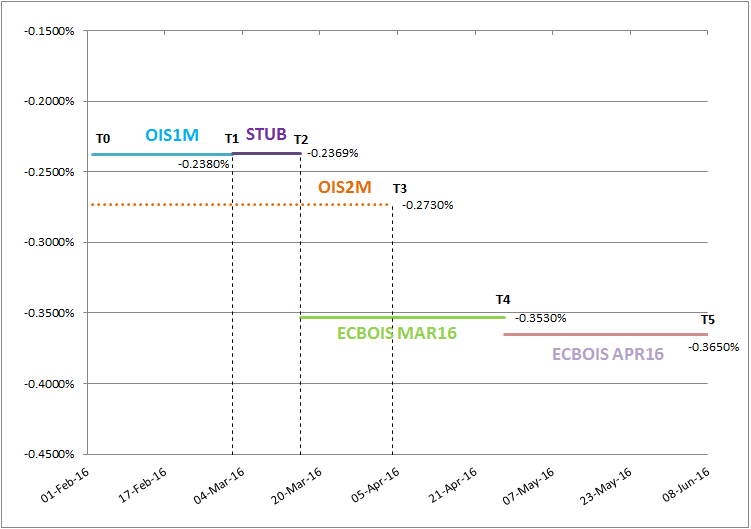
\includegraphics[width=0.75\textwidth]{stubsol.png}
\caption{La stesso scenario mostrato nella Figura \ref{fig:overlappingsol} applicando lo Stub.}
\label{fig:stubsol}
\end{figure}
\end{tframe}
%%%%%%%%%%%%%%%%%%%%%%%%%%%%%%%%%%%%%%%%%%%%%%%%%%%%%%%%%%%%%
\begin{tframe}{Impatto sugli errori di repricing}
\begin{figure}[!h]
\centering
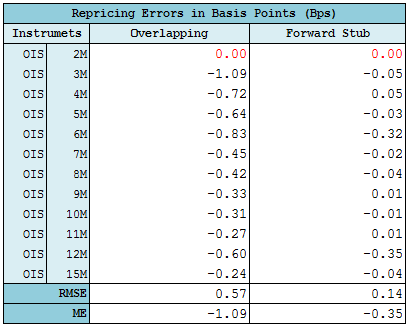
\includegraphics[width=0.55\textwidth]{errors.png}
\caption{Riassunto degli errori di repricing relativi a strumenti fuori curva per entrambe le soluzioni.}
\label{fig:errors}
\end{figure}
\end{tframe}
%%%%%%%%%%%%%%%%%%%%%%%%%%%%%%%%%%%%%%%%%%%%%%%%%%%%%%%%%%%%%
\begin{tframe}{Forma funzionale della curva overnight}
\begin{itemize}
\item I fixings dell'indice EONIA tendono ad avere un'andamento particolare
   \begin{itemize}
   \item Essi sono infatti costanti a tratti tra date di incontro del consiglio di politica monetaria della BCE
   \item Tuttavia assumere un'andamento dei tassi costante a tratti anche nel lungo periodo sarebbe un'enorme incoerenza
   \end{itemize}
\item Modellare coerentemente la curva overnight presuppone di tenere conto di queste peculiarità della shape
\item Il problema si riduce alla scelta del miglior schema di interpolazione in grado di riprodurne l'andamento
\end{itemize}
\end{tframe}
%%%%%%%%%%%%%%%%%%%%%%%%%%%%%%%%%%%%%%%%%%%%%%%%%%%%%%%%%%%%%
\begin{tframe}
\begin{figure}[!h]
\centering
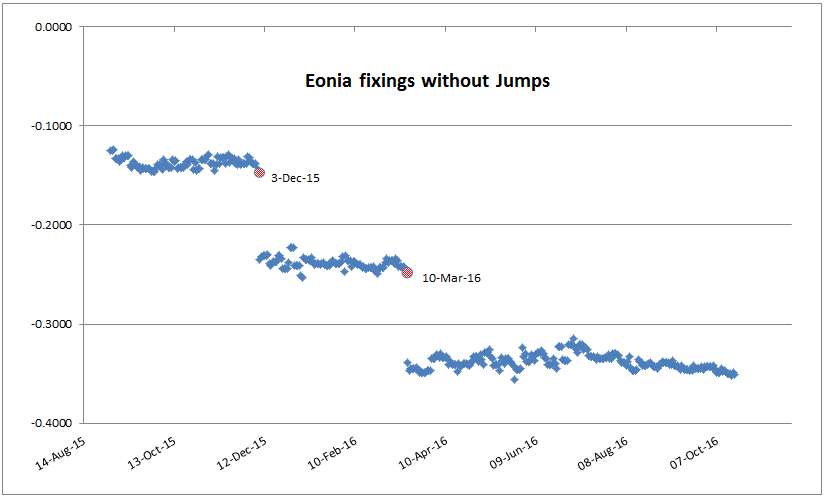
\includegraphics[width=0.8\textwidth]{eoniafixings.png}
\caption{Andamento costante a tratti dei fixings dell'indice EONIA per l'ultimo anno}
\label{fig:eoniafixings}
\end{figure}
\end{tframe}
%%%%%%%%%%%%%%%%%%%%%%%%%%%%%%%%%%%%%%%%%%%%%%%%%%%%%%%%%%%%%
\begin{tframe}
\begin{itemize}
\item Poichè usare un'interpolazione lineare per tutta la curva è sconsigliabile, la best practice converge verso l'utilizzo di interpolazioni cubiche le quali producono tassi forward smooth.
\item Tuttavia queste tecniche conducono a due problemi:
   \begin{itemize}
   \item Non hanno un buon fit con la shape della curva nel breve termine la quale dovrebbe essere costante a tratti
   \item L'algoritmo proposto per il Forward Stub non sarebbe più coerente poichè assume tassi flat tra date di meeting della BCE
   \item Tuttavia è comunque possibile ricavare la quota implicita anche con interpolazione cubica attraverso un meccanismo di root finding.
   \end{itemize}
\item La soluzione proposta è quella di creare un nuovo schema di interpolazione, detto {\it Interpolazione Mista}, che unisca due schemi diversi di interpolazione
\item In questo modo è possibile usare un'interpolazione lineare per il breve termine per poi passare ad un'interpolazione cubica per il medio/lungo termine
\end{itemize}
\end{tframe}
%%%%%%%%%%%%%%%%%%%%%%%%%%%%%%%%%%%%%%%%%%%%%%%%%%%%%%%%%%%%%
\begin{tframe}
\begin{figure}[!h]
\centering
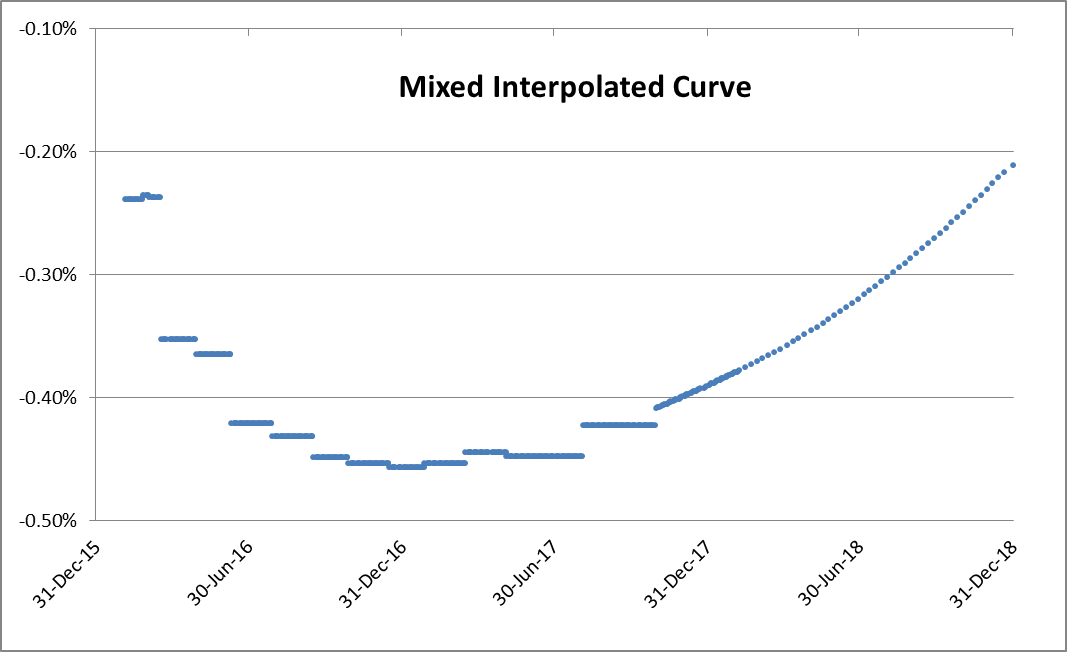
\includegraphics[width=0.75\textwidth]{splitrange.png}
\caption{Un esempio di curva costruita unendo un'interpolazione lineare sui log-discount fino alla fine della strip di ECB OIS e un'interpolazione cubica monotona in seguito.}
\label{fig:splitrange}
\end{figure}
\end{tframe}
%%%%%%%%%%%%%%%%%%%%%%%%%%%%%%%%%%%%%%%%%%%%%%%%%%%%%%%%%%%%%
\begin{tframe}{Impatto sugli errori di repricing}
\begin{figure}[!h]
\centering
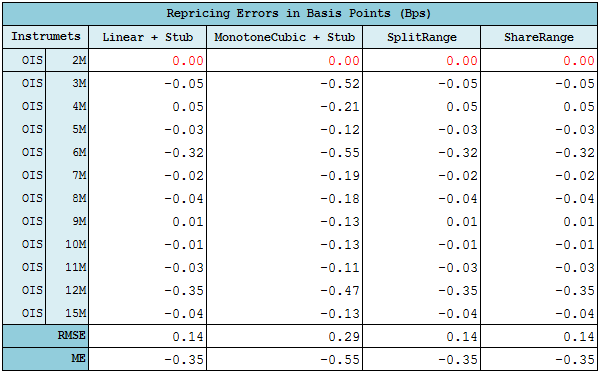
\includegraphics[width=0.70\textwidth]{repricingmixed.png}
\caption{Riassunto degli errori di repricing relativi a strumenti fuori curva per tutte le soluzioni analizzate.}
\label{fig:repricingmixed}
\end{figure}
\end{tframe}
%%%%%%%%%%%%%%%%%%%%%%%%%%%%%%%%%%%%%%%%%%%%%%%%%%%%%%%%%%%%%
\begin{tframe}{Jump e Turn-Of-Year ({\it TOY}) effects}
\begin{itemize}
\item Il punto chiave per ottenere una curva calibrata allo stato dell'arte è ottenere tassi forward smooth
\item Anche scegliere il miglior schema di interpolazione possibile può non essere sufficiente se prima della calibrazione non si escludono tutti i market rate jumps per poi includerli nuovamente una volta ottenuta la curva.
\item In termini di grandezza il jumps più rilevante è il cosìdetto Turn-Of-Year effect, osservabile nelle quotazioni di mercato il cui tenore scavalca l'anno. 
\item Da un punto di vista finanziario il TOY effect è dovuto alla crescente/decrescente ricerca di liquidità causata dai requisiti di capitale regolamentari e dalla necessità di chiudere i bilanci annuali.
\end{itemize}
\end{tframe}
%%%%%%%%%%%%%%%%%%%%%%%%%%%%%%%%%%%%%%%%%%%%%%%%%%%%%%%%%%%%%
\begin{tframe}
\begin{itemize}
\item L'indice EONIA mostra jump {\bfseries positivi} di size variabile quasi tutti i fine mese
\end{itemize}
\begin{figure}[!h]
\centering
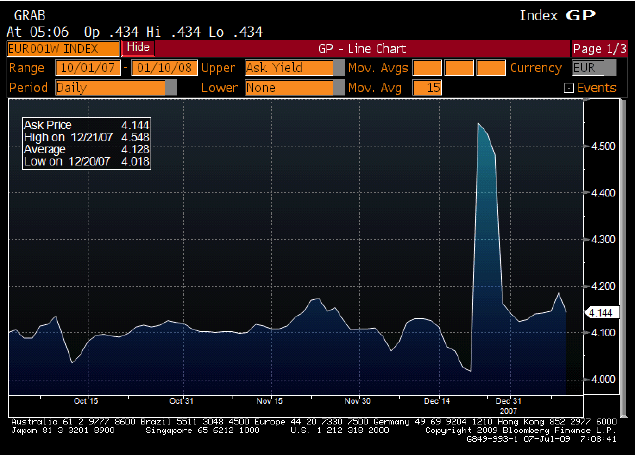
\includegraphics[width=0.65\textwidth]{turnofyear.png}
\caption{Il TOY effect di fine Dicembre 2014 visto dal terminale Bloomberg.}
\label{fig:turnofyear}
\end{figure}
\end{tframe}
%%%%%%%%%%%%%%%%%%%%%%%%%%%%%%%%%%%%%%%%%%%%%%%%%%%%%%%%%%%%%
\begin{tframe}
\begin{itemize}
\item Il Fed Funds rate presenta jump {\bfseries negativi} praticamente ogni fine mese e di size particolarmente rilevanti
\end{itemize}
\begin{figure}[!h]
\centering
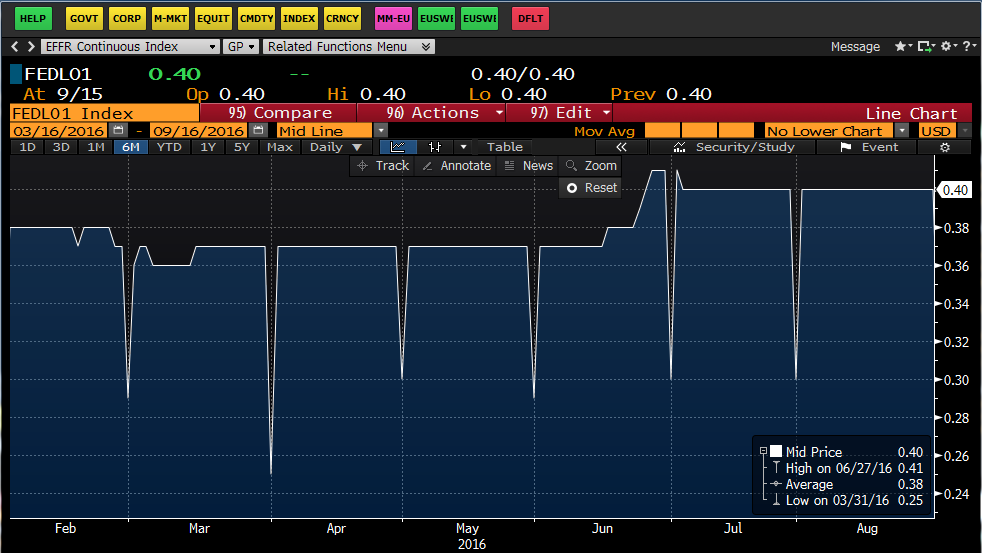
\includegraphics[width=0.75\textwidth]{bloombergusd.png}
\caption{I jumps degli ultimi 7 mesi visti dal terminale Bloomberg}
\label{fig:bloombergusd}
\end{figure}
\end{tframe}
%%%%%%%%%%%%%%%%%%%%%%%%%%%%%%%%%%%%%%%%%%%%%%%%%%%%%%%%%%%%%
\begin{tframe}{Jump estimation}
\begin{itemize}
\item Al fine di stimare la size, negativa o positiva, dei jump si propone un'approcio a 4 step simile a quello proposto da Burghardt (\cite{burg}):
   \begin{enumerate}
   \item Costruire una curva overnight calibrando tutti gli strumenti liquidi disponibili e usando un'interpolazione flat sui forward rates
   \item Stimare il primo jump assumendo che il segmento fuori linea risposto al precedente e successivo possa essere rimesso in linea scaricando la differenza nel jump; quindi se il jump è positivo:
   $$\left[F^{Original}(t\ped{1},t\ped{2}) - F^{Interp}(t\ped{1},t\ped{2})\right] \cdot \tau(t\ped{1},t\ped{2}) = J^{Size}*\tau^{J}$$
   se invece è negativo:
   $$\left[F^{Interp}(t\ped{1},t\ped{2}) - F^{Original}(t\ped{1},t\ped{2})\right] \cdot \tau(t\ped{1},t\ped{2}) = J^{Size}*\tau^{J}$$
   \item Eliminare dalla curva il jump trovato al punto precedente
   \item Ripetere il punto 2 e 3 alla prossima data di jump
   \end{enumerate}
\end{itemize}
\end{tframe}
%%%%%%%%%%%%%%%%%%%%%%%%%%%%%%%%%%%%%%%%%%%%%%%%%%%%%%%%%%%%%
\begin{tframe}{Jump estimation}
\begin{itemize}
\item Al fine di stimare la size, negativa o positiva, dei jump si propone un'approcio a 4 step simile a quello proposto da Burghardt (\cite{burgh}):
\end{itemize}
\end{tframe}
%%%%%%%%%%%%%%%%%%%%%%%%%%%%%%%%%%%%%%%%%%%%%%%%%%%%%%%%%%%%%
\begin{tframe}{Jump estimation}
\begin{itemize}
\item Al fine di stimare la size, negativa o positiva, dei jump si propone un'approcio a 4 step simile a quello proposto da Burghardt (\cite{burgh}):
   \begin{enumerate}
   \item Costruire una curva overnight calibrando tutti gli strumenti liquidi disponibili e usando un'interpolazione flat sui forward rates
   \end{enumerate}
\end{itemize}
\end{tframe}
%%%%%%%%%%%%%%%%%%%%%%%%%%%%%%%%%%%%%%%%%%%%%%%%%%%%%%%%%%%%%
\begin{tframe}{Jump estimation}
\begin{itemize}
\item Al fine di stimare la size, negativa o positiva, dei jump si propone un'approcio a 4 step simile a quello proposto da Burghardt (\cite{burgh}):
   \begin{enumerate}
   \item Costruire una curva overnight calibrando tutti gli strumenti liquidi disponibili e usando un'interpolazione flat sui forward rates
   \item Stimare il primo jump assumendo che il segmento fuori linea risposto al precedente e successivo possa essere rimesso in linea scaricando la differenza nel jump; quindi se il jump è positivo:
   $$\left[F^{Original}(t\ped{1},t\ped{2}) - F^{Interp}(t\ped{1},t\ped{2})\right] \cdot \tau(t\ped{1},t\ped{2}) = J^{Size}*\tau^{J}$$
   se invece è negativo:
   $$\left[F^{Interp}(t\ped{1},t\ped{2}) - F^{Original}(t\ped{1},t\ped{2})\right] \cdot \tau(t\ped{1},t\ped{2}) = J^{Size}*\tau^{J}$$
   \end{enumerate}
\end{itemize}
\end{tframe}
%%%%%%%%%%%%%%%%%%%%%%%%%%%%%%%%%%%%%%%%%%%%%%%%%%%%%%%%%%%%%
\begin{tframe}{Jump estimation}
\begin{itemize}
\item Al fine di stimare la size, negativa o positiva, dei jump si propone un'approcio a 4 step simile a quello proposto da Burghardt (\cite{burgh}):
   \begin{enumerate}
   \item Costruire una curva overnight calibrando tutti gli strumenti liquidi disponibili e usando un'interpolazione flat sui forward rates
   \item Stimare il primo jump assumendo che il segmento fuori linea risposto al precedente e successivo possa essere rimesso in linea scaricando la differenza nel jump; quindi se il jump è positivo:
   $$\left[F^{Original}(t\ped{1},t\ped{2}) - F^{Interp}(t\ped{1},t\ped{2})\right] \cdot \tau(t\ped{1},t\ped{2}) = J^{Size}*\tau^{J}$$
   se invece è negativo:
   $$\left[F^{Interp}(t\ped{1},t\ped{2}) - F^{Original}(t\ped{1},t\ped{2})\right] \cdot \tau(t\ped{1},t\ped{2}) = J^{Size}*\tau^{J}$$
   \item Eliminare dalla curva il jump trovato al punto precedente
   \end{enumerate}
\end{itemize}
\end{tframe}
%%%%%%%%%%%%%%%%%%%%%%%%%%%%%%%%%%%%%%%%%%%%%%%%%%%%%%%%%%%%%
\begin{tframe}{Jump estimation}
\begin{itemize}
\item Al fine di stimare la size, negativa o positiva, dei jump si propone un'approcio a 4 step simile a quello proposto da Burghardt (\cite{burgh}):
   \begin{enumerate}
   \item Costruire una curva overnight calibrando tutti gli strumenti liquidi disponibili e usando un'interpolazione flat sui forward rates
   \item Stimare il primo jump assumendo che il segmento fuori linea risposto al precedente e successivo possa essere rimesso in linea scaricando la differenza nel jump; quindi se il jump è positivo:
   $$\left[F^{Original}(t\ped{1},t\ped{2}) - F^{Interp}(t\ped{1},t\ped{2})\right] \cdot \tau(t\ped{1},t\ped{2}) = J^{Size}*\tau^{J}$$
   se invece è negativo:
   $$\left[F^{Interp}(t\ped{1},t\ped{2}) - F^{Original}(t\ped{1},t\ped{2})\right] \cdot \tau(t\ped{1},t\ped{2}) = J^{Size}*\tau^{J}$$
   \item Eliminare dalla curva il jump trovato al punto precedente
   \item Ripetere il punto 2 e 3 alla prossima data di jump
   \end{enumerate}
\end{itemize}
\end{tframe}
%%%%%%%%%%%%%%%%%%%%%%%%%%%%%%%%%%%%%%%%%%%%%%%%%%%%%%%%%%%%%
\begin{tframe}
\begin{figure}[!h]
\centering
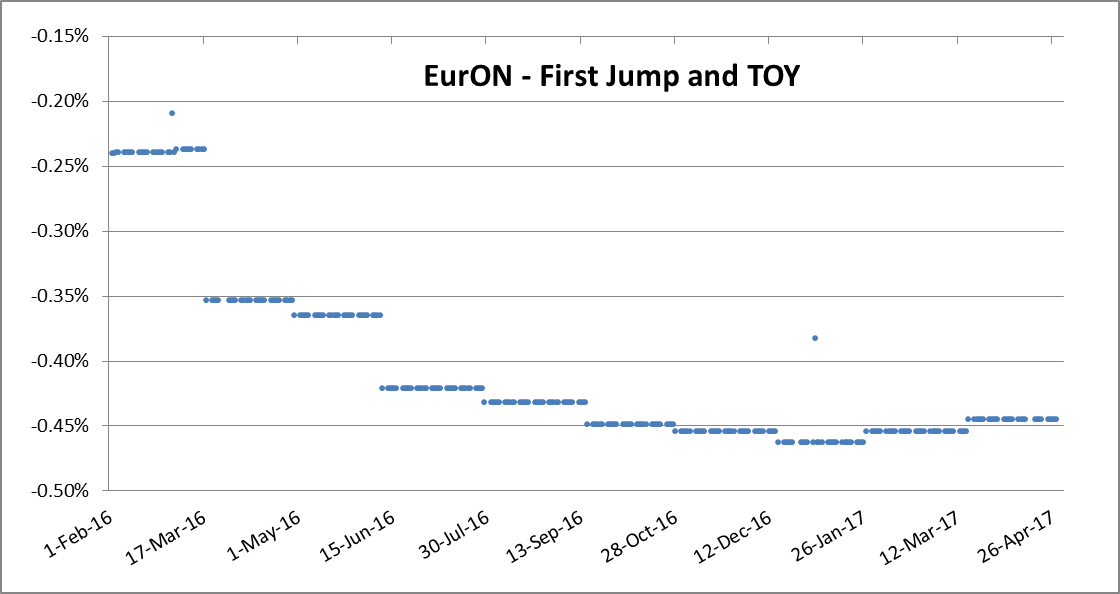
\includegraphics[width=0.8\textwidth]{firstjumpeur3.png}
\caption{Prima parte della curva EUR overnight calibrata togliendo jump e TOY e inserendoli a fine calibrazione.}
\label{fig:firstjumpeur3}
\end{figure}
\end{tframe}
%%%%%%%%%%%%%%%%%%%%%%%%%%%%%%%%%%%%%%%%%%%%%%%%%%%%%%%%%%%%%
\begin{tframe}
\begin{figure}[!h]
\centering
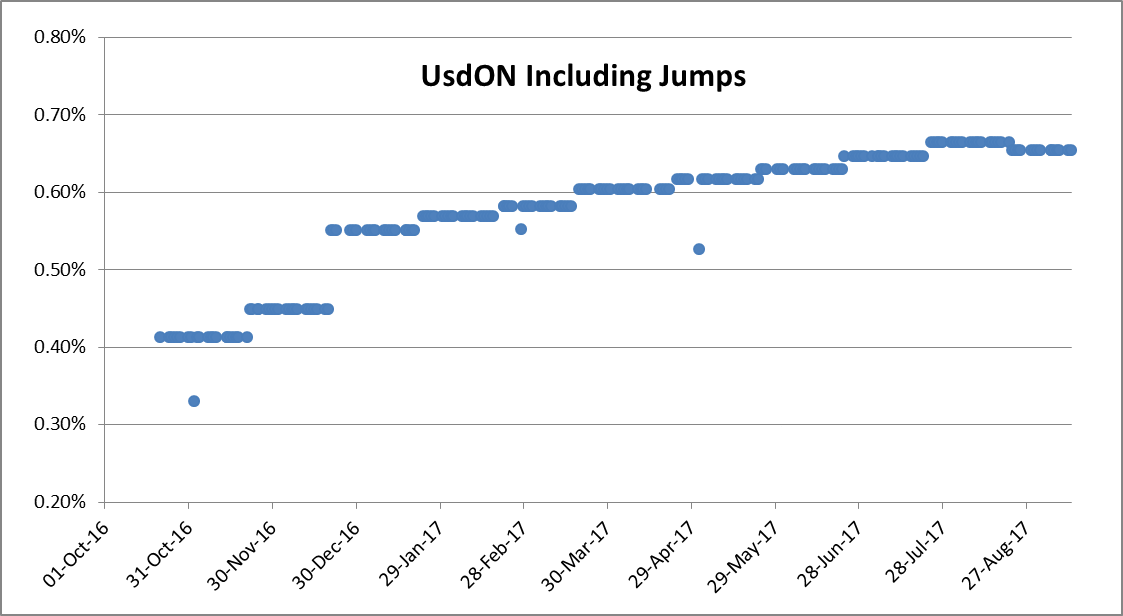
\includegraphics[width=0.8\textwidth]{firstjumpusd3.png}
\caption{Prima parte della curva USD overnight calibrata togliendo tutti i jump stimati e inserendoli a fine calibrazione.}
\label{fig:firstjumpusd3}
\end{figure}
\end{tframe}
%%%%%%%%%%%%%%%%%%%%%%%%%%%%%%%%%%%%%%%%%%%%%%%%%%%%%%%%%%%%%